
\subsection{Experimentaci\'on 2: Red de oficina}

\subsubsection{Descripci\'on del contexto}
El experimento fue realizado en una red de ámbito laboral. Se trata de una pequeña empresa de desarrollo web que cuenta con 13 empleados, los cuales utilizan una computadora de escritorio o notebook además de dispositivos móviles. La oficina cuenta con un servidor en donde mantine alojados los archivos de producción dentro de repositorios locales y donde los empleados suben modificaciones de los archivos constantemente.

\subsubsection{Descripci\'on de la captura}
Los resultados presentados a continuación se coresponden con la captura de paquetes de la red durante un intervalo de 3 horas.
Se capturó un total de 392521 paquetes, de los cuales 1715 fueron del tipo ARP.
\begin{itemize}
\item IP version 6: 3.67\%
\item ARP: 0.564\%
\item DOD Internet Protocol (IP): 95.7627%
\end{itemize}
Se puede observar que sólo se capturó 3 tipos de paquetes, de los cuales en su gran mayoría son del tipo DOD Internet Protocol (IP).
A contuniación se exhibe una comparación entre paquetes IP versión 6 y ARP, pudiendose observar que la cantidad de paquetes del tipo IP versión 6 es ampliamente mayor que la del tipo ARP.
\begin{center}
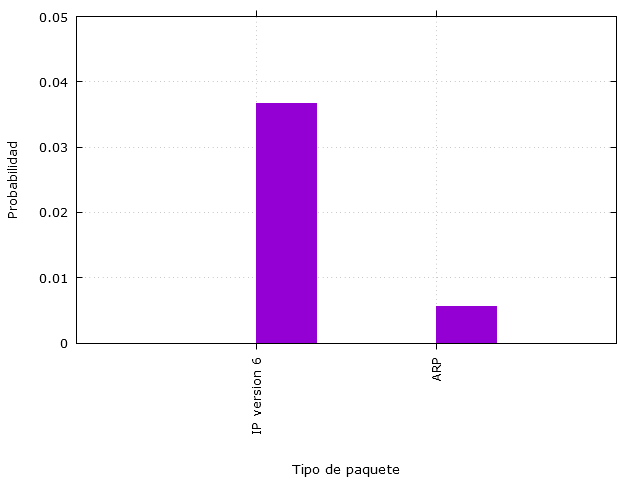
\includegraphics[width=0.5\textwidth]{exp2-graficos/grafico1exp2.png}
\end{center}

La entrop\'ia de la fuente S fue: 0.277044626815.\newline

Tomando los paquetes ARP se puede distinguir las direcciones IP en 34 diferentes, lo cual es un número razonable tiendo en cuenta la cantidad de terminales aproximada.

A continuación vemos un histograma con todas las direcciones IP observadas y la cantidad de paquetes hacia estas.

\begin{center}
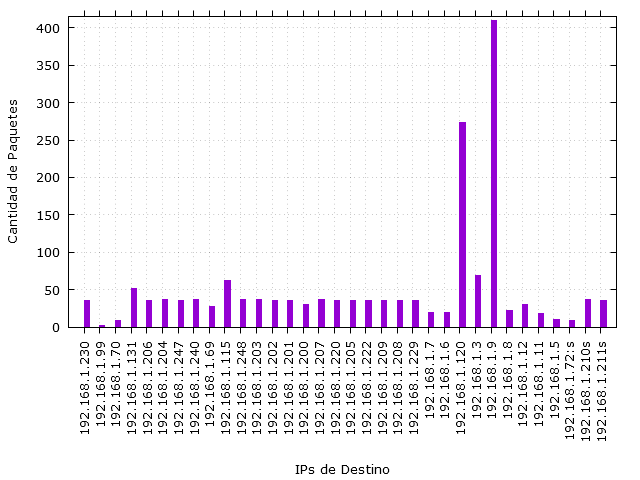
\includegraphics[width=0.75\textwidth]{exp2-graficos/grafico2exp2.png}
\end{center}

La entrop\'ia de la fuente S1 fue: 4.2739682572.


\subsubsection{An\'alisis de la captura}
Fuente S:
Como vimos en el 1er histograma, el 95$%$ de los paquetes fueron de tipo IPv4, lo que muestra que en la red hay un alto uso de paquetes de datos.

En cuanto a la entropía de la fuente es de 0.277 con lo cual se
puede ver que es más bien baja. Basandonos en la teoría de la información podemos ver que la probabilidad de un símbolo del tipo IP acapara la mayoria de la fuente, logrando que uno pueda inferir que si uno toma un símbolo emitido por la fuente este va a ser del tipo IP casi con seguridad.

Fuente S1:
Al mirar el segundo histograma, se puede observar que las IPs más distinguidas resultan ser claramente la 192.168.1.9 y 192.168.1.120. La 192.168.1.9 resulta ser el servidor mencionado.


